% ============================================================
%  深圳大学实验报告模板（SZU Experiment Report Template）
% This template can be modified according to the specific requirements of your experiment or project.
% Produced by: Chao Fan and Kewei Ou, AI School of SZU
% ============================================================

\documentclass[a4paper,12pt]{article}

% ----------------------------
% 中文与字体支持
% ----------------------------
\usepackage{fontspec}    % 字体支持
\usepackage{xeCJK}       % 中文字体支持
\IfFontExistsTF{Noto Serif CJK SC}
    {\setCJKmainfont{Noto Serif CJK SC}}
    {\setCJKmainfont[AutoFakeBold=2]{SimSun}}

\IfFontExistsTF{Noto Serif CJK SC}
    {\setCJKmonofont{Noto Serif CJK SC}}
    {\setCJKmonofont[AutoFakeBold=2]{SimSun}}

% 图中使用的两个标注命令
\newcommand{\shp}[1]{{\footnotesize\ttfamily\color{black!55}#1}}
\newcommand{\todotag}[1]{{\scriptsize\bfseries\color{red!70!black}#1}}

% ----------------------------
% 页面设置与常用宏包
% ----------------------------
\usepackage{geometry}    % 页面边距控制
\geometry{left=1in, right=1in, top=1in, bottom=1in}
\setlength{\parindent}{2em}
\setlength{\parskip}{0pt}

\usepackage{longtable}   % 支持长表格
\usepackage{graphicx}    % 插入图片
\usepackage{fancyhdr}    % 页眉页脚控制
\usepackage{tikz}        % 绘制框线等图形
\usetikzlibrary{calc, positioning, arrows.meta, backgrounds, fit}
\usepackage{verbatim}    % 显示代码块
\usepackage{float}       % 控制图片浮动位置（[H]参数）
\usepackage{amsmath}     % 公式
\usepackage{amssymb}     % \mathbb 等符号
\usepackage{booktabs}    % 三线表
\usepackage{xcolor}      % 颜色
\usepackage{listings}    % 代码高亮
\usepackage{lstlinebgrd} % 按行加底色，用于标出关键代码
\usepackage{caption}     % 图表标题格式
\usepackage{needspace}   % 避免代码块被拆到两页
\usepackage{xurl}        % 允许网址在任意位置断行

\renewcommand{\figurename}{图}
\renewcommand{\tablename}{表}
\captionsetup{font=small, labelsep=quad}
\renewcommand{\arraystretch}{1.12}
\setlength{\emergencystretch}{2em}

% ----------------------------
% 代码块样式
% ----------------------------
\definecolor{codebg}{RGB}{248,248,250}
\definecolor{markbg}{RGB}{255,244,214}

% 给指定行加底色：\hl{行号}
\newcommand{\hl}[1]{\ifnum\value{lstnumber}=#1 \color{markbg}\fi}

\lstdefinestyle{numpy}{
    language=Python,
    basicstyle=\ttfamily\footnotesize,
    keywordstyle=\color[RGB]{30,80,160}\bfseries,
    commentstyle=\color[RGB]{30,120,70}\itshape,
    backgroundcolor=\color{codebg},
    frame=single,
    rulecolor=\color{black!20},
    framerule=0.4pt,
    framesep=4pt,
    xleftmargin=10pt,
    xrightmargin=6pt,
    showstringspaces=false,
    columns=fullflexible,
    keepspaces=true,
    breaklines=true,
    aboveskip=5pt,
    belowskip=5pt,
}
\lstset{style=numpy}

% ----------------------------
% 页眉页脚设置
% ----------------------------
% \pagestyle{fancy}
\fancyhf{} % 清空默认页眉页脚
% \fancyhead[L]{深圳大学实验报告} % 左侧页眉文字
\fancyhead[C]{} % 中间空
\fancyhead[R]{} % 右侧空

% ============================================================
%                      文档开始
% ============================================================

\begin{document}

% ============================================================
% 封面页
% ============================================================
\begin{titlepage}
    \centering
    \vspace*{2cm}
    \Huge{\textbf{深 \ 圳 \ 大 \ 学 \ 实 \ 验  \ 报 \ 告}}\\[1.5cm]
    
    {\Large\textbf{课程名称}\quad\underline{\makebox[8cm][c]{Python程序设计}}}\\[0.5cm]
{\Large
\noindent\makebox[3.2cm][l]{\textbf{项目名称}}
\underline{\makebox[8cm][c]{project1-numpy}}}\\[0.5cm]
{\Large
\noindent\makebox[3.2cm][l]{\textbf{学 \quad \quad 院}}
\underline{\makebox[8cm][c]{人工智能学院}}}\\[0.5cm]
{\Large
\noindent\makebox[3.2cm][l]{\textbf{专 \quad \quad 业}}
\underline{\makebox[8cm][c]{人工智能}}}\\[0.5cm]
{\Large
\noindent\makebox[3.2cm][l]{\textbf{指导教师}}
\underline{\makebox[8cm][c]{舒婷}}}\\[0.5cm]
{\Large
\noindent\makebox[3.2cm][l]{\textbf{报 \quad 告 \quad 人}}
\underline{\makebox[3cm][c]{黄英桐}}
\hspace{0.5cm}
\textbf{学号}
\underline{\makebox[3cm][c]{2025681014}}}\\[0.5cm]
{\Large
\noindent\makebox[3.2cm][l]{\textbf{实验时间}}
\underline{\makebox[8cm][c]{2026/11/19}}}\\[0.5cm]
{\Large
\noindent\makebox[3.2cm][l]{\textbf{提交时间}}
\underline{\makebox[8cm][c]{2026/11/19}}}\\[1.5cm]

    \vfill
    \Large{\textbf{教务处制}}
\end{titlepage}

\newpage

% ============================================================
% 正文部分
% ============================================================

\section{实验目的}

用 NumPy 实现 OpenCLIP ViT-B/32 的图像编码器前向：补全 \texttt{image\_encoder.py} 的 TODO-01 至 TODO-06，把 $[B,3,224,224]$ 算成每张图一个 512 维单位向量。参数、预处理和数值辅助函数由课程提供，不训练，不用 GPU 和 PyTorch。验收看四点：形状一致、类型为 \texttt{float32}、数值有限、逐元素误差满足 $|\hat{y}-y|\le \mathrm{atol}+\mathrm{rtol}\,|y|$；内部 token 取 $\mathrm{atol}=2\times10^{-4}$，输出取 $2\times10^{-5}$，$\mathrm{rtol}=2\times10^{-4}$，输出每行长度还要为 1。

\section{实现}

模型 12 层、宽 768、12 头各 64 维；$224\times224$ 按 $32\times32$ 切成 49 块，每块 3072 个数，加 CLS 共 50 个 token，MLP 中间层 3072 维。图~\ref{fig:vit-arch} 是前向流程，橙色为本次实现。

\begin{figure}[htbp]
    \centering
    \begin{tikzpicture}[
        node distance=3.4mm,
        box/.style={draw, rounded corners=2pt, minimum height=8mm,
                    text width=8.0cm, align=center, font=\footnotesize,
                    inner sep=3pt},
        mine/.style={box, fill=orange!10, draw=red!65!black, line width=0.8pt},
        given/.style={box, fill=blue!6, draw=blue!45!black, line width=0.5pt},
        ar/.style={-{Latex[length=2mm,width=1.6mm]}, line width=0.7pt, draw=black!55},
      ]
      \node[given] (n1) {预处理后的 RGB 图像\\[1pt]\shp{[B, 3, 224, 224]}};
      \node[mine, below=of n1] (n2) {切分并展平图块\quad\todotag{TODO-01}\\[1pt]\shp{[B, 49, 3072]}};
      \node[mine, below=of n2] (n3) {图块投影、拼接 CLS、加位置编码\quad\todotag{TODO-05}\\[1pt]\shp{[B, 50, 768]}};
      \node[given, below=of n3] (n4) {输入 LayerNorm\\[1pt]\shp{[B, 50, 768]}};
      \node[mine, below=of n4, text width=8.7cm] (n5)
        {\textbf{Transformer block $\times$ 12}\quad\todotag{TODO-02 / 03 / 04}\\[1pt]
         拆头 $\to$ 注意力 $\to$ 合头 $\to$ 残差 $\to$ MLP $\to$ 残差\\[1pt]
         \shp{[B, 50, 768] 保持不变}};
      \node[mine, below=of n5] (n6) {取 CLS、后置 LayerNorm、线性投影\quad\todotag{TODO-06}\\[1pt]
         \shp{[B, 768] $\to$ [B, 512]}};
      \node[given, below=of n6] (n7) {L2 归一化（课程提供）\\[1pt]\shp{float32 [B, 512]}};

      \foreach \a/\b in {n1/n2, n2/n3, n3/n4, n4/n5, n5/n6, n6/n7}
        \draw[ar] (\a) -- (\b);

      \begin{scope}[on background layer]
        \node[draw=red!65!black, dashed, line width=0.5pt, rounded corners=3pt,
              inner sep=3pt, fit=(n2)(n3)] (g1) {};
        \node[draw=red!65!black, dashed, line width=0.5pt, rounded corners=3pt,
              inner sep=3pt, fit=(n5)(n6)] (g2) {};
      \end{scope}
      \node[font=\scriptsize\bfseries, text=red!70!black, anchor=west]
            at ($(g1.east)+(3pt,0)$) {本次实现};
      \node[font=\scriptsize\bfseries, text=red!70!black, anchor=west]
            at ($(g2.east)+(3pt,0)$) {本次实现};

      \node[given, minimum height=4.5mm, text width=1.9cm, font=\scriptsize,
            anchor=north west] at ($(n7.south west)+(-0.1,-0.40)$) {课程提供};
      \node[mine, minimum height=4.5mm, text width=1.9cm, font=\scriptsize,
            anchor=north west] at ($(n7.south west)+(2.2,-0.40)$) {本次实现};
      \node[font=\scriptsize, text=black!60, anchor=north west]
            at ($(n7.south west)+(4.5,-0.15)$) {括号内为张量形状，$B$ 为图像数};
    \end{tikzpicture}
    \caption{图像编码器的前向流程。蓝色为课程提供的计算，橙色为本次补全的步骤。}
    \label{fig:vit-arch}
\end{figure}

\noindent\textbf{切块与嵌入。}六轴 \texttt{reshape} 把图像拆成 batch、通道、$7\times7$ 网格和块内像素，\texttt{transpose} 把网格轴提到通道轴前，最后一次 \texttt{reshape} 展平。patch 顺序完全由轴序决定，写反不报错，只会在 \texttt{patches} 阶段对不上。嵌入把每块投到 768 维（无偏置），拼上 CLS，再加位置编码，位置编码没有 batch 轴，靠广播相加。

\needspace{8\baselineskip}
\begin{lstlisting}[linebackgroundcolor={\hl{2}}]
x = images.reshape(B, 3, 7, 32, 7, 32)
x = x.transpose(0, 2, 4, 1, 3, 5)          # 轴序决定 patch 排列
return x.reshape(B, 49, 3072)

tokens = patches @ self.patch_weight.T
cls = np.repeat(self.cls, images.shape[0], axis=0)
tokens = np.concatenate((cls, tokens), axis=1)
tokens += self.position
\end{lstlisting}

\noindent\textbf{多头注意力。}拆头把 768 维分成 12 组、每组 64 维，再把 head 轴移到 token 轴前：每个 head 看到全部 50 个 token，但只处理自己那 64 维。分数按 $\mathrm{scores}=qk^{\mathsf{T}}/\sqrt{d_h}$ 算，除 $\sqrt{64}=8$ 是为了点积不随维度变大而让 softmax 饱和；系数由课程提供的 \texttt{attention\_weights} 归一化得到，乘 $v$ 后合头、投影。

\needspace{8\baselineskip}
\begin{lstlisting}[linebackgroundcolor={\hl{1}\hl{3}}]
k_t = k.transpose(0, 1, 3, 2)              # 只换最后两轴
scores = q @ k_t
scores = scores / np.sqrt(np.float32(self.head_dim))   # 用 float32 开方

coefficients = attention_weights(scores)
context = coefficients @ v
context = context.transpose(0, 2, 1, 3)
merged = context.reshape(B, N, D)
output = merged @ self.out_weight.T + self.out_bias
\end{lstlisting}

\noindent\textbf{block 与输出头。}预归一化结构，先归一化再算，结果加回输入，两条残差都保持 $[B,50,768]$；MLP 先扩到 3072 维，过 GELU 再缩回。输出头只取第 0 行 CLS，过 \texttt{post\_norm} 和 $[768,512]$ 投影，最后单位化。

\needspace{8\baselineskip}
\begin{lstlisting}[linebackgroundcolor={\hl{6}\hl{9}}]
residual = x + update
u = self.norm2(residual)
hidden = u @ self.fc1_weight.T + self.fc1_bias
hidden = self.gelu(hidden)
mlp_update = hidden @ self.fc2_weight.T + self.fc2_bias   # 3072 -> 768
return residual + mlp_update

cls = tokens[:, 0, :]
cls = self.post_norm(cls)
return unit_vector(cls @ self.projection)   # 权重已是 [in, out]
\end{lstlisting}

权重按 PyTorch 的 $[\text{out},\text{in}]$ 存放，乘法前要转置；只有 \texttt{visual.proj} 已是 $[768,512]$，不能再转。

\section{结果}

项目目录下执行 \verb|python check.py --stage all|，8 个阶段全部通过，输出见图~\ref{fig:check}，各阶段误差见表~\ref{tab:errors}。环境为 Python 3.13.7、NumPy 2.5.5、Pillow 12.3.0。

\begin{figure}[htbp]
    \centering
    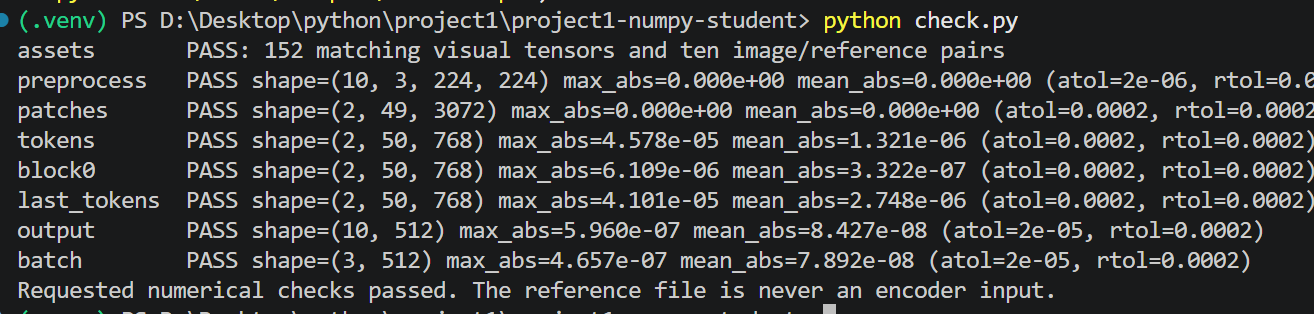
\includegraphics[width=0.88\linewidth]{check_output.png}
    \caption{8 个阶段全部 PASS；终端右侧被截断的容差列见表~\ref{tab:errors}。}
    \label{fig:check}
\end{figure}

\begin{table}[htbp]
    \centering
    \caption{各阶段相对参考数组的误差}
    \label{tab:errors}
    \small
    \begin{tabular}{lcrrr}
        \toprule
        阶段 & 输出形状 & 最大绝对误差 & 平均绝对误差 & 相对 L2 误差 \\
        \midrule
        \texttt{preprocess}   & $[10,3,224,224]$ & $0$ & $0$ & $0$ \\
        \texttt{patches}      & $[2,49,3072]$    & $0$ & $0$ & $0$ \\
        \texttt{tokens}       & $[2,50,768]$     & $4.578\times10^{-5}$ & $1.321\times10^{-6}$ & $1.18\times10^{-6}$ \\
        \texttt{block0}       & $[2,50,768]$     & $6.109\times10^{-6}$ & $3.322\times10^{-7}$ & $2.22\times10^{-6}$ \\
        \texttt{last\_tokens} & $[2,50,768]$     & $4.101\times10^{-5}$ & $2.748\times10^{-6}$ & $4.34\times10^{-6}$ \\
        \texttt{output}       & $[10,512]$       & $5.960\times10^{-7}$ & $8.427\times10^{-8}$ & $2.48\times10^{-6}$ \\
        \texttt{batch}        & $[3,512]$        & $4.657\times10^{-7}$ & $7.892\times10^{-8}$ & $2.34\times10^{-6}$ \\
        \bottomrule
    \end{tabular}
\end{table}

\texttt{preprocess} 和 \texttt{patches} 只做缩放、切片、重排，没有浮点累加，误差为 0。进入矩阵乘法后误差在 $10^{-6}$ 到 $10^{-5}$，来自 BLAS 与参考实现的分块累加顺序不同；\texttt{last\_tokens} 没有随 12 层放大，因为 LayerNorm 把特征拉回固定尺度，残差又让主分量直接透传。\texttt{output} 反而最小，是 L2 归一化把每行缩到长度 1、幅值只有 $0.044$，绝对误差跟着变小，实测每行长度 $0.99999994$ 到 $1.0$，与参考的余弦相似度不低于 $0.99999994$。\texttt{batch} 把顺序改成 $[1,0,1]$ 后仍逐行对齐，说明没有缓存参考结果，样本之间也不互相影响。

\section{讨论}

注意力分数最初写成 \verb|scores / np.sqrt(self.head_dim)|：\texttt{head\_dim} 是 Python 整数，\verb|np.sqrt| 返回 \texttt{float64}，\texttt{float32} 数组相除会被提升，最终输出不再是 \texttt{float32}。除数先转 \texttt{float32} 再开方，因子仍是 $8$，类型保持。按 \texttt{float64} 重算整条前向，数值差只有 $1.32\times10^{-7}$，能过数值容差，但类型不符照样判失败——验收查的是接口契约。

$k$ 是四维数组，\texttt{k.T} 会把四个轴全颠倒，\texttt{q @ k.T} 直接抛 \texttt{ValueError}，只能交换最后两轴；\texttt{mlp.c\_proj.weight} 存成 $[768,3072]$，漏写 \texttt{.T} 同样报错；\texttt{visual.proj} 已是 $[768,512]$，不能再转。三处都是方向问题，只有一处不转。

验证只覆盖课程给的 10 张图和 3 种 batch 组合，没试边界输入；GELU 用逐元素循环，$B=10$ 时可以接受，但不是最快的写法。

\section{个人贡献与协助}

六个 TODO 的输入输出形状是我逐个推的，实现和调试也是我做的；注意力缩放的类型问题是核对输出类型时发现并改的，MLP 第二层漏掉的 \texttt{.T} 是对照权重形状补上的。外部协助用于理解多头注意力和 MLP 的组织方式、核对 NumPy 写法，报告的排版与流程图有 AI 参与。权重、预处理、辅助函数、检查脚本和参考数组由课程提供，未改动。

提交 \texttt{image\_encoder.py}、README 和本报告。生成结果用 \texttt{python run.py}，参数 \texttt{--output output\_tokens.npz}，按输入顺序导出 10 张图的 ID 与特征。代码仓库：\url{https://github.com/ach3rry/project1-vit-numpy}。

\newpage

% ============================================================
% 批阅与成绩评定页
% ============================================================

% 绘制正文外框（包含批阅区域）
\begin{tikzpicture}[remember picture, overlay]
  \draw[thick] 
    ($(current page.north west)+(2cm,-3cm)$) 
    rectangle 
    ($(current page.south east)+(-2cm,3.5cm)$);
\end{tikzpicture}

\vspace{1cm}

% 批阅区
\noindent \textbf{指导教师批阅意见：}
\vspace{6cm}
\hfill

\vspace{1cm}

\noindent \textbf{成绩评定：}
\vspace{2cm}
\hfill

\vspace{1cm}

\noindent
\hfill
\textbf{指导教师签字：}\quad\quad\quad\quad\quad\\[0.5cm]

\hfill
\textbf{年}\quad\quad
\textbf{月}\quad\quad
\textbf{日}\quad

\vspace{1cm}

% 备注部分
\noindent \textbf{备注：}

% 框外的注释
\begin{tikzpicture}[remember picture, overlay]
  \node[
    anchor=north west,
    inner sep=0pt,
    text width=\dimexpr\paperwidth-4cm\relax
  ] at ($(current page.south west)+(2cm,3.1cm)$) {
    \begin{minipage}{\dimexpr\paperwidth-4cm\relax}
      \small
      \noindent
      \textbf{注：}\;1、报告内的项目或内容设置，可根据实际情况加以调整和补充。\\[0.2cm]
      \phantom{\textbf{注：}\;}2、教师批改学生实验报告时间应在学生提交实验报告时间后 10 日内。
    \end{minipage}
  };
\end{tikzpicture}

% ============================================================
%                      文档结束
% ============================================================

\end{document}
